%%%%%%%%%%%%%%%%%%%%%%%%%%%%%%%%%%%%%%%%%
% Jacobs Landscape Poster
% LaTeX Template
% Version 1.0 (29/03/13)
%
% Created by:
% Computational Physics and Biophysics Group, Jacobs University
% https://teamwork.jacobs-university.de:8443/confluence/display/CoPandBiG/LaTeX+Poster
% 
% Further modified by:
% Nathaniel Johnston (nathaniel@njohnston.ca)
%
% This template has been downloaded from:
% http://www.LaTeXTemplates.com
%
% License:
% CC BY-NC-SA 3.0 (http://creativecommons.org/licenses/by-nc-sa/3.0/)
%
%%%%%%%%%%%%%%%%%%%%%%%%%%%%%%%%%%%%%%%%%

%----------------------------------------------------------------------------------------
%	PACKAGES AND OTHER DOCUMENT CONFIGURATIONS
%----------------------------------------------------------------------------------------

\documentclass[final]{beamer}

\usepackage[scale=1.24]{beamerposter} % Use the beamerposter package for laying out the poster
\usepackage{algorithmic}

\usetheme{confposter} % Use the confposter theme supplied with this template

\setbeamercolor{block title}{fg=ngreen,bg=white} % Colors of the block titles
\setbeamercolor{block body}{fg=black,bg=white} % Colors of the body of blocks
\setbeamercolor{block alerted title}{fg=white,bg=dblue!70} % Colors of the highlighted block titles
\setbeamercolor{block alerted body}{fg=black,bg=dblue!10} % Colors of the body of highlighted blocks
% Many more colors are available for use in beamerthemeconfposter.sty

%-----------------------------------------------------------
% Define the column widths and overall poster size
% To set effective sepwid, onecolwid and twocolwid values, first choose how many columns you want and how much separation you want between columns
% In this template, the separation width chosen is 0.024 of the paper width and a 4-column layout
% onecolwid should therefore be (1-(# of columns+1)*sepwid)/# of columns e.g. (1-(4+1)*0.024)/4 = 0.22
% Set twocolwid to be (2*onecolwid)+sepwid = 0.464
% Set threecolwid to be (3*onecolwid)+2*sepwid = 0.708

\newlength{\sepwid}
\newlength{\onecolwid}
\newlength{\twocolwid}
\newlength{\threecolwid}
\setlength{\paperwidth}{48in} % A0 width: 46.8in
\setlength{\paperheight}{36in} % A0 height: 33.1in
\setlength{\sepwid}{0.024\paperwidth} % Separation width (white space) between columns
\setlength{\onecolwid}{0.30\paperwidth} % Width of one column
\setlength{\twocolwid}{0.65\paperwidth} % Width of two columns
\setlength{\topmargin}{-0.5in} % Reduce the top margin size
%-----------------------------------------------------------

\usepackage{graphicx}  % Required for including images

\usepackage{booktabs} % Top and bottom rules for tables

%----------------------------------------------------------------------------------------
%	TITLE SECTION 
%----------------------------------------------------------------------------------------

\title{Incentivizing Exploration By Heterogeneous Users} % Poster title

\author{Bangrui Chen\footnotemark[1], Peter I. Frazier\footnotemark[1] \& David Kempe\footnotemark[2]} % Author(s)

\institute{\footnotemark[1] School of Operations Research and Information Engineering, Cornell University; \footnotemark[2] Department of Computer Science, USC} % Institution(s)

%----------------------------------------------------------------------------------------

\begin{document}

\addtobeamertemplate{block end}{}{\vspace*{2ex}} % White space under blocks
\addtobeamertemplate{block alerted end}{}{\vspace*{2ex}} % White space under highlighted (alert) blocks

\setlength{\belowcaptionskip}{2ex} % White space under figures
\setlength\belowdisplayshortskip{2ex} % White space under equations

\begin{frame}[t] % The whole poster is enclosed in one beamer frame

\begin{columns}[t] % The whole poster consists of three major columns, the second of which is split into two columns twice - the [t] option aligns each column's content to the top

\begin{column}{\sepwid}\end{column} % Empty spacer column

\begin{column}{\onecolwid} % The first column


\begin{block}{Motivation}
\begin{center}
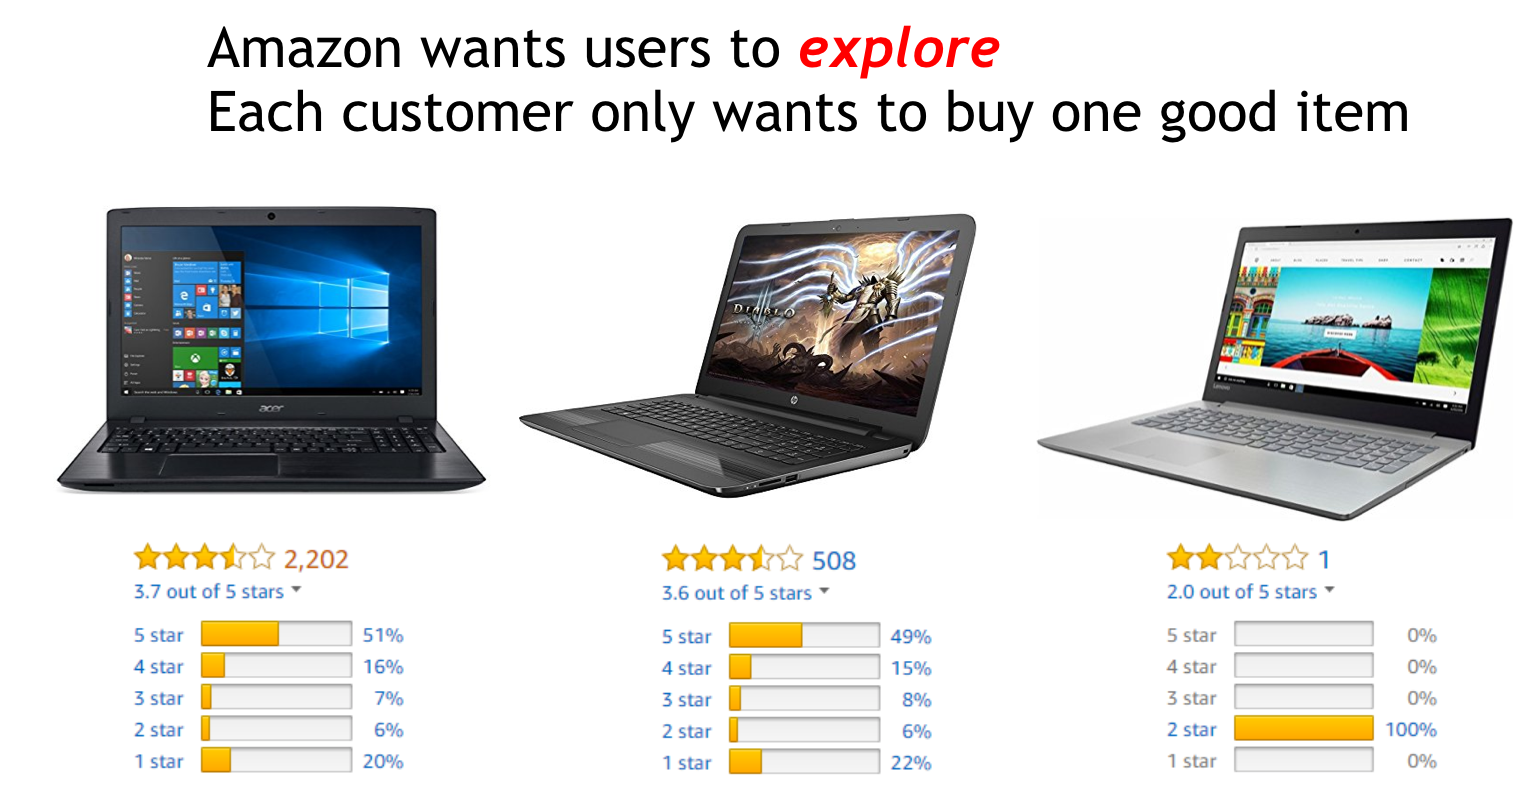
\includegraphics[scale=1]{example}
\end{center}

An alternative that seems worse initially may remain unexplored because customers have no incentives to explore it!
\end{block}

\begin{block}{Literature Review}
Two recent lines of work have shown that effecting a societally near-optimal outcome in this setting requires explicitly inducing exploration:
\begin{itemize}
\item \textbf{Without Money Transfer} Kremer et al. (2014) and Mansour et al. (2015, 2016, 2018) assume that the principal has an informational advantage in being the only one to observe the results of past arm pulls (as in driving route recommendations). The principal can use her advantage to induce exploration by recommending apparently sub-optimal arms, as long as agents cannot do better on their own.
\item \textbf{With Money Transfer} Frazier et al. (2014) and Han et al. (2015) instead assume that the results of all past arm pulls are publicly observable (as on a review-sharing site). They suppose that the principal can incentivize exploration by offering arm-specific reward payments.
\end{itemize}
In this work, we present the first algorithm/analysis for incentivizing exploration when users have heterogeneous preferences over arms and we prove \textbf{“heterogeneity provides free exploration"}.
\end{block}

\begin{block}{Model}
\begin{itemize}
\item $N$ bandit arms provide vector-valued outcomes equal to an unknown arm-specific attribute vector $u_{i}\in \mathbb{R}^{d}$, perturbed by independent noise. 
\item Agents arrive sequentially and observe current estimates of the arms’ attribute vectors $\hat{u}_{i,t}$, which are averages of other agents’ past pulls. 
\item Agents have heterogeneous linear preferences over arm attributes.
\item Agent $t$ has preference vector $\theta_t$ drawn from a known distribution.
\item A principal knows only the distribution from which agents’ preferences are drawn but not the specific draws.
\item The principal can offer arm-specific incentive payments $c_{t,i}$ to encourage agents to explore underplayed arms. 
\item Agents are myopic and choose the arm $i_t = \arg\max_{i}\{\theta_{t}\cdot \hat{u}_{i,t} + c_{t,i_t}\}$.
\item The regret at time $t$ is $r_t = (\max_{i} \theta_t \cdot u_i) - \theta_t \cdot u_{i_t}$ and the payment is $c_t = c_{t,i_t}$.
\item The principal seeks to minimize the total expected cumulative regret while also making a small expected cumulative payment.
\end{itemize}
\end{block}

\end{column} % End of the first column

\begin{column}{\sepwid}\end{column} % Empty spacer column
\begin{column}{\onecolwid} % The first column


\begin{block}{Key Assumptions}

\begin{itemize}
\item (\textbf{Every arm is someone's best}) We use $p$ to denote the minimum (over all arms) fraction of users that prefer any particular arm.
\item (\textbf{Not too many near-ties}) Let $q(z)$ be the cumulative distribution function of those agents whose utility difference between their best and second best arm is less than or equal to $z$, then there exists a $\hat{z}>0$, $L$ such that $q(z)\leq L\cdot z$ for all $z\leq \hat{z}$.
\item (\textbf{Compact Support}) $\theta$ has a compact support set contained in $[0,D]^{d}$.
\end{itemize}

\end{block}


\begin{block}{Main Results}
\begin{alertblock}{Theorem 1}
With the previously stated assumptions, there is a policy that achieves expected 
cumulative regret $O (N e^{2/p} + L N \log^3(T))$,
using expected cumulative payments of $O(N^2 e^{2/p})$.
\newline
\newline
In particular, when agents who are close to tied between two arms have measure $0$,
both the expected regret and expected payment are bounded by constants
(with respect to $T$). 
\end{alertblock}
\end{block}

\begin{block}{Algorithm}


\textbf{Notation:}
\vspace{0.5cm}
\begin{itemize}
\item Phase: Phase $s$ starts when each arm has been pulled at least $s$ times. $m_{t,i}$ denotes the number of pulls for arm $i$ up to time $t$. 
\item Payment-eligible: An arm $i$ is \emph{payment-eligible} at time $t$ (in phase $s$) if both of the following hold:
\begin{itemize}
\item $i$ has been pulled at most $s$ times up to time $t$, i.e., $m_{t,i} \leq s$.
\item  The conditional probability of pulling arm $i$ is less than$1/\log(s)$ given the current estimates $\hat{u}_{t,i'}$ of the arms' attribute vectors.  
\end{itemize}
\end{itemize}


\vspace{0.5cm}
\textbf{Our Algorithm:}
\vspace{0.5cm}

\begin{algorithmic}
\STATE Set the current phase number $s = 1$.
\COMMENT{Each arm is pulled once initially ``for free.''}
\FOR{time steps $t = 1, 2, 3, \ldots$} {
\IF {$m_{t,i} \geq s+1$ for all arms $i$}
\STATE Increment the phase $s = s + 1$.
\ENDIF
\IF {there is a payment-eligible arm $i$} 
    \STATE Let $i$ be an arbitrary payment-eligible arm.
    \STATE Offer payment $c_{t,i} = \max_{\theta,i'} \theta \cdot (\hat{\mu}_{t,i'} - \hat{\mu}_{t,i})$ for pulling arm $i$ (and payment 0 for all other arms).
\ELSE
    \STATE Let agent $t$ play myopically, i.e., offer payments 0 for all arms.
\ENDIF 
}\ENDFOR
\end{algorithmic}

\end{block}
		
%----------------------------------------------------------------------------------------
\end{column}

\begin{column}{\sepwid}\end{column} % Empty spacer column

\begin{column}{\onecolwid} % The second column within column 2 (column 2.2)


\begin{block}{Proof Sketch}
The key technical lemma in our proof is a Hoeffding-like concentration inequality that holds for a random, adaptively chosen number of samples (Zhao et al. 2016).

\vspace{1cm}

\textbf{Payment Proof:}
\begin{itemize}
\item For the early phases, we crudely bound the number of payment by $N$ for each phase;
\vspace{0.3cm}
\item For the later phases, we uses our technical lemma to rule out any incentives unless large misestimates of the arm locations occur, which is exponentially unlikely as the phase advances.
\end{itemize}

\vspace{1cm}

\textbf{Regret Proof:}
\begin{itemize}
\item Regret incurred when an agent was incentivized to pull a sub-optimal arm: the analysis here is very similar to the payment proof;
\vspace{0.5cm}
\item Regret incurred when an agent myopically pulled a suboptimal arm: in this case, we define a phase-dependent cutoff $\gamma(s(t))$ to distinguish agents based on their regret.
\vspace{0.3cm}
\begin{itemize}
\item Agents with $r(t)\geq \gamma(s(t))$:
\begin{itemize}
\item this requires severe misestimates of arm locations and such misestimates are exponentially unlikely to occur;
\vspace{0.1cm}
\item since $\theta_t$ has a compact support, the maximum regret is bounded by a constant;
\end{itemize}
\vspace{0.3cm}
\item Agents with $r(t)\leq \gamma(s(t))$: 
\begin{itemize}
\item this requires agents to be almost tied in their preference for the best arm, but there are not so many agents have near-ties preferences;
\vspace{0.1cm}
\item the maximum regret is bounded above by $\gamma(s(t))$;
\end{itemize}
\end{itemize}
\end{itemize}
\vspace{1cm}


\end{block}
\begin{block}{References}
[1] Ilan Kremer, Yishay Mansour, and Motty Perry. Implementing the “wisdom of the crowd”. Journal of Political Economy, 122(5):988–1012, 2014. \newline
[2] Yishay Mansour, Aleksandrs Slivkins, and Vasilis Syrgkanis. Bayesian incentive-compatible bandit exploration. In Proceedings of the 16th ACM Conference on Economics and Computation (EC), pages 565–582. ACM, 2015. \newline
[3] Yishay Mansour, Aleksandrs Slivkins, Vasilis Syrgkanis, and Zhiwei Steven Wu. Bayesian explo- ration: Incentivizing exploration in bayesian games. In Proceedings of the 17th ACM Conference on Economics and Computation (EC), 2016. \newline
[4] Yishay Mansour, Aleksandrs Slivkins, and Zhiwei Steven Wu. Bayesian exploration: Incentivizing exploration in bayesian games. In Proceedings of the 9th Innovations in Theoretical Computer Science (ITCS) conference, 2018. \newline
[5] Peter Frazier, David Kempe, Jon Kleinberg, and Robert Kleinberg. Incentivizing exploration. In Proceedings of the 15th ACM conference on Economics and Computation (EC), pages 5–22. ACM, 2014. \newline
[6] Li Han, David Kempe, and Ruixin Qiang. Incentivizing exploration with heterogeneous value of money. In Proceedings of the 11th International Conference on Web and Internet Economics (WINE), pages 370–383. Springer, 2015. \newline
[7] Shengjia Zhao, Enze Zhou, Ashish Sabharwal, and Stefano Ermon. Adaptive concentration inequal- ities for sequential decision problems. In Proceedings of the 30th Advances In Neural Information Processing Systems (NIPS), pages 1343–1351, 2016.
\end{block}

%----------------------------------------------------------------------------------------

\end{column} % End of column 2.2


\begin{column}{\sepwid}\end{column} % Empty spacer column

\begin{column}{\onecolwid} % The third column

%----------------------------------------------------------------------------------------

\end{column} % End of the third column

\end{columns} % End of all the columns in the poster

\end{frame} % End of the enclosing frame

\end{document}
